\section{Maple to Semantic \LaTeX{} Translator}\label{sec:backward-translation}
The backward translation is based on the internal data structure of \Maple. Therefore, a license of \Maple{} is mandatory to perform backward translations. The following subsections will explain why this approach was necessary and how \Maple{} works internally. Using the internal data structure also requires to handle the internal properties of \Maple. This can causes some problems. Those problems and our solutions will be explained in subsection~\ref{subsec:maple-probs}. In the last subsection~\ref{subsec:maple-impl}, we will focus on the implementation of the backward translation.

Note that all explanations in this section is based on \Maple's programming guide~\cite{MAPLE:ProgrammingGuide} for \Maple{} 2016. 

\subsection{Internal Data Structure}
While our forward translation is realized for the \texttt{1D} input representation in \Maple, this representation is not suitable for a backward translation. Since \Maple{} uses it's own syntax and programming language, we would need a new parser for \Maple{} expressions to realize a backward translation tool. Of course, \Maple{} has this parser implemented. But it is not possible to use the parser without using \Maple{} itself. Therefore, an installed version of \Maple{} is mandatory for our backward translation.  

As already mentioned, \Maple{} has several ways to represent an expression. The \texttt{1D} and \texttt{2D} representations are used as input representations. Besides those, there are internal data structures to perform all kinds of computations on the expression. Internally, each expression is handled and stored as a \gls{dag}. The \Maple{} \gls{dag} is very similar to an expression tree. But for efficiency, it does not store copies of an object. Consider the integral from (\ref{eq:maple-input})
\begin{equation}\label{eq:maple-input-2}
\int\displaylimits_0^\infty \frac{\pi+\sin(2x)}{x^2} dx.
\end{equation}

As already mentioned, the \Maple{} \gls{dag} has no copies of objects. Therefore, the '$x$' in \eqref{eq:maple-input-2} only appears once in the \gls{dag}.
\begin{figure}[ht]
\centering
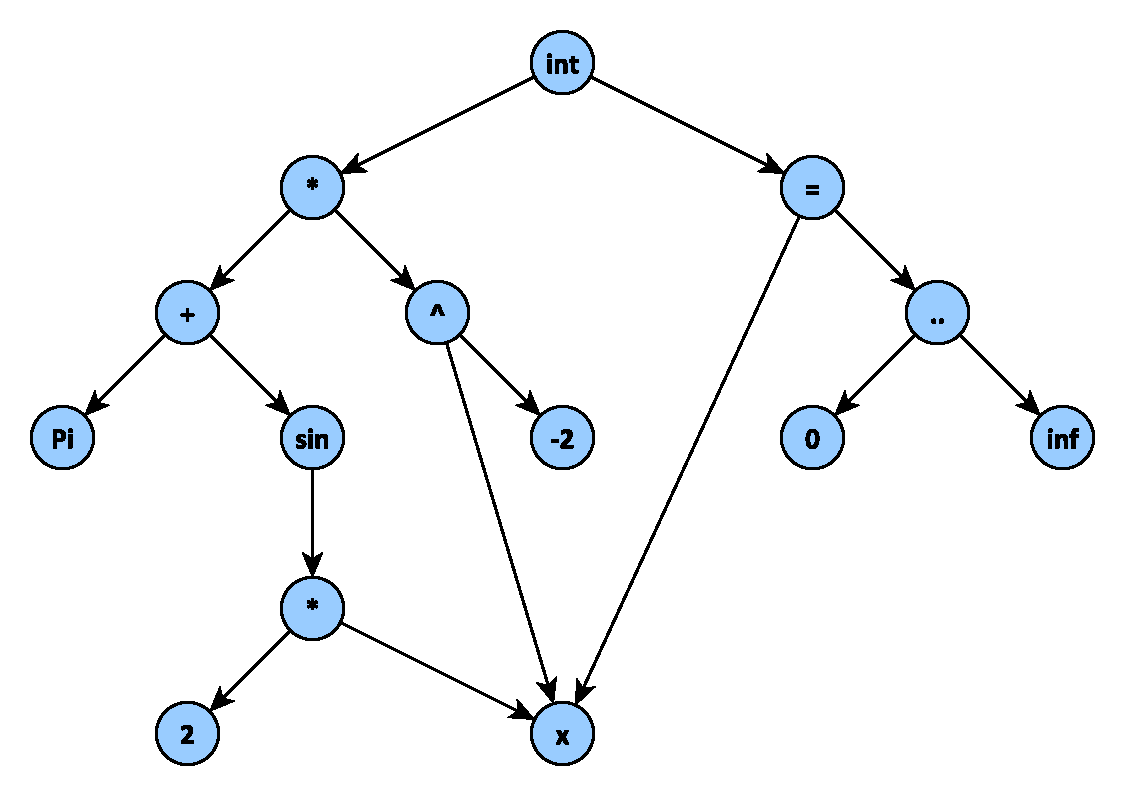
\includegraphics[scale=0.7]{DAG.pdf}
\caption{The \Maple{} DAG of equation~\eqref{eq:maple-input}}
\label{fig:maple-dag}
\end{figure}

The \Maple{} \gls{dag} can be visualized in a graph, such as in figure~\ref{fig:maple-dag}. But the internal representation looks a bit different. Each node in the \gls{dag} stores its children and has a header, which defines the type and the length of the node. Consider the polynomial $x^2+x$. Figure~\ref{fig:internal-maple-dag} illustrates the internal \gls{dag} representation with headers and arguments.

\begin{figure}[ht]
	\centering
	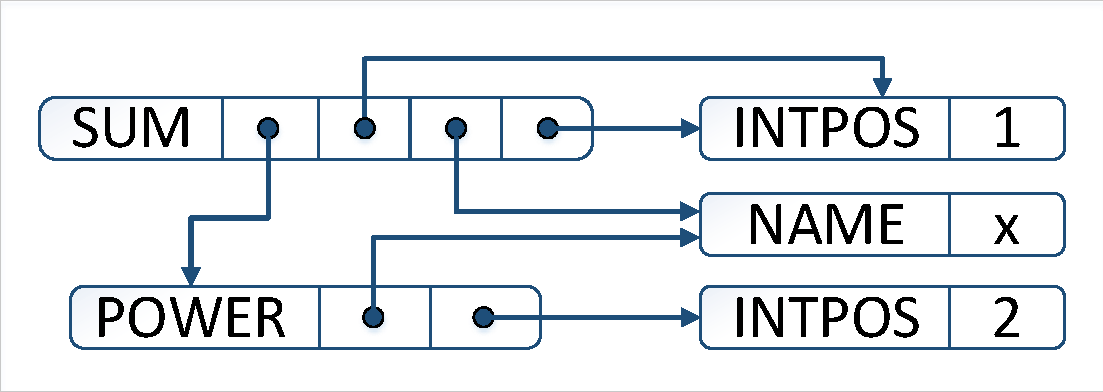
\includegraphics[clip, trim=0.1cm 0.1cm 0.1cm 0.1cm, scale=0.7]{DAGreal.pdf}
	\caption{The internal \Maple{} DAG representation of $x^2+x$.}
	\label{fig:internal-maple-dag}
\end{figure}

\Maple{} has also another representation, similar to the \gls{dag}, that allows multiple copies of the same object in its representation. This representation is called \inertF{} and is more similar to an expression tree than \Maple's \gls{dag}. The \inertF{} represents the \gls{dag} as a tree by splitting object copies and displays the tree in a list structure. Each node (or element in the list) has the prefix \texttt{\_Inert\_XXX}, that indicates the node is in the \inertF. The suffix \texttt{XXX} is the type of the node. Some of the important types are specified in table~\ref{tab:maple-types}. Note that this is only a subset of all possible types.

\begin{table}[ht]
\centering
\begin{tabular}{cp{10cm}}
	\hline
	Type & Explanation\\
	\hline
	SUM & Sums.\\
	PROD & Products.\\
	EXPSEQ & Expression sequence is a kind of list. The arguments of functions are stored in such sequences.\\
	INTPOS & Positive integers.\\
	INTNEG & Negative integers.\\
	COMPLEX & Complex numbers with real and imaginary part.\\
	FLOAT & Float numbers are stored in the scientific notation with integer values for the exponent $n$ and the significand $m$ in $m \cdot 10^n$.\\
	RATIONAL & Rational numbers are fractions stored in integer values for the numerator and positive integers for the denominator.\\
	POWER & Exponentiation with expressions as base and exponent.\\
	FUNCTION & Function invocation with the name, arguments and attributes of the function.\\
	\hline
\end{tabular}
\caption{A subset of important internal \Maple{} structures. See~\cite{MAPLE:ProgrammingGuide} for a complete list.}
\label{tab:maple-types}
\end{table}

\subsection{Maple's Open Maple API}
\Maple{} provides an \gls{api}, called \texttt{OpenMaple}~\cite[\S 14.3]{MAPLE:ProgrammingGuide} for interaction with the \Maple{} kernel. The \texttt{OpenMaple} \gls{api} is implemented for different programming languages such as \texttt{C}, \texttt{Java} and \texttt{Visual Basic}. Since our forward translation and the \gls{mlp} is implemented in \texttt{Java}, we use the \texttt{Java} \gls{api} for the backward translation. The \texttt{Java} \gls{api} has some limitations to interact with \Maple's \gls{dag}.

For the backward translation, we use the \inertF. This representation can be converted to a nested list version and the \texttt{OpenMaple} Java \gls{api} can handle lists. Therefore, the backward translation firstly converts the \inertF{} to a nested list structure before any translation process starts.

The following figure~\ref{fig:inertform-list} shows the \inertF{} and the nested list of the polynomial $x^2+x$.

\begin{figure}[ht]
\centering
\begin{minipage}{.45\linewidth}
\centering
\begin{tabular}{lll}
\multicolumn{3}{l}{\_Inert\_SUM(}\\
& \multicolumn{2}{l}{\_Inert\_POWER(}\\
& & \_Inert\_NAME("x"),\\
& & \_Inert\_INTPOS(2)\\
& ),\\ 
& \multicolumn{2}{l}{\_Inert\_NAME("x")}\\
)
\end{tabular}
\end{minipage}
\begin{minipage}{.45\linewidth}
\centering
\begin{tabular}{lll}
\multicolumn{3}{l}{[\_Inert\_SUM,}\\
& \multicolumn{2}{l}{[\_Inert\_POWER, }\\
& & [\_Inert\_NAME, "x"],\\
& & [\_Inert\_INTPOS, 2]\\
& ],\\ 
& \multicolumn{2}{l}{[\_Inert\_NAME, "x"]}\\
]
\end{tabular}
\end{minipage}
\caption{\inertF{} and the nested list representation of $x^2+x$.}
\label{fig:inertform-list}
\end{figure}

In the nested list, the first element specifies the type of the current list while the following arguments store the arguments and optional attributes.

\subsection{Workarounds for Problems}\label{subsec:maple-probs}
Note that the backward translations usually do not have problems with ambiguous expressions. Every \gls{cas} needs to solve ambiguities in its own representation, otherwise it could not compute the expression. Our backward translation from \Maple{} back to semantic \LaTeX{} is therefore based on already disambiguated expressions.

The general walkthrough of our backward translation starts with a string of a \texttt{1D} \Maple{} input expression. As described above, this string is entered in \Maple{} to parse the expression and work on the nested list version of the \inertF{} afterwards. This causes some problems. Mostly because \Maple{} automatically evaluates input expressions immediately - even before we have a chance to take a look at the internal data structure of the input. For example, an input such as $\sin@{\frac{\cpi}{2}}$ is immediately evaluated to $1$ and the internal data structure just shows us the positive integer value $1$ instead of the trigonometric function.

Furthermore, \Maple{} also changes input expressions slightly, mostly because of missing data types for a specific expression. For example, the internal data structure has no type to represent fractions except the \texttt{RATIONAL} type, which only allows integer values for the numerator and denominator. Thereby, an expression like $\frac{x}{2}$ is automatically changed to $x\frac{1}{2}$. There is no way no avoid such simple arithmetic changes in the expression, but we can avoid the automatic evaluations.

Firstly, we summarize all known changes and evaluations \Maple{} automatically performs on input expressions.

\begin{itemize}
\item \Maple{} evaluates input expressions immediately.
\item There is no data type to represents square roots such as $\sqrt{x}$ (or $n$-th roots). Therefore, \Maple{} stores roots as an exponentiation with a fractional exponent. For example, $\sqrt{x}$ is stored as $x^{\frac{1}{2}}$.
\item There is no data type for subtractions, only for sums. Negative terms are changed to absolute values times '$-1$'. For example, $x-y$ is stored as $x + y \cdot (-1)$. 
\item Floating point numbers are stored in the scientific notation with a mantissa and an exponent in the base $10$. For example, $3.1$ is internally represented as $31 \cdot 10^{-1}$.
\item There is only a data type for rational numbers (fractions with integer numerator and positive denominator), but not for general fractions, such as $\frac{x+y}{z}$. This will be automatically changed to $(x+y)\cdot z^{-1}$.
\end{itemize}

There are unevaluation quotes implemented to avoid evaluations on input expression. Table~\ref{tab:unevaluation-quotes} gives an example how those unevaluation quotes work.

\begin{table}[ht]
\centering
\begin{tabular}{lcc}
\hline
& Without unevaluation quotes & With unevalation quotes\\
\hline
Input expression: & \texttt{sin(Pi)+2-1} & \texttt{'sin(Pi)+2-1'}\\
Stored expression: & 1 & \texttt{sin(Pi)+1}\\
\hline
\end{tabular}
\caption{Example of unevaluation quotes for \texttt{1D} \Maple{} input expressions.}
\label{tab:unevaluation-quotes}
\end{table}

Since we want to keep a translated expression similar to the input expression, we use unevaluation quotes during the whole translation process. Unevaluation quotes also solve the problems with square roots and $n$-th roots. In \Maple's \texttt{1D} input representation, a square root is a function call (\texttt{sqrt(x)}) and the unevaluation quotes prevent evaluations on functions. Therefore, a backward translation simply needs to translate a square root as a normal function. Hence, we do not have problems with the internal representation of roots in \Maple.

Because of the absent data type for subtractions, a long sum with negative terms could be difficult to read. We change the order of constants (such as an integer value) to be in front of products. Therefore, an expression such as '$-y$' is not represented by '$y\cdot (-1)$', but by '$(-1) \cdot y$'. The translator now needs to check if there is a leading '$-1$' and can translate it to '$-y$' rather than to '$(-1) \cdot y$'.

Floating point numbers in scientific notation also causes a problem. Consider the input expression $0.41$ as the nested list \inertF{} representation
\begin{equation}
\texttt{[\_Inert\_FLOAT, [\_Inert\_INTPOS, 41], [\_Inert\_INTNEG, 2]]}.
\end{equation}

The backward translator is implemented in \texttt{Java}. To translate such an expression back to $0.41$, computations become necessary. Of course, it makes sense to perform those computations in the \gls{cas} (in that case, in \Maple) rather than in the translation program. Therefore, we implemented a procedure\footnote{\textit{Procedures} in \Maple{} are small programs similar to methods and functions in \gls{oop} languages.} to automatically convert \texttt{FLOAT} nodes to a string representation of the floating point number. We created a new type, called \texttt{MYFLOAT} to represent such numbers. With this approach, we avoided computations in the translation process.

For fractions, we use a similar approach and introduce a new internal data type \texttt{DIVIDE}. The implementation of \texttt{DIVIDE} was difficult. On the one hand, some expressions with negative exponent should be displayed as a fraction while others should should be displayed with the negative exponent. We follow the same rule as \Maple{} follows internally to display fractions. When the exponent is a negative numeric element, the expression should be displayed as a fraction. If the exponent is something else, we uses the negative exponent representation. Table~\ref{tab:maple-fracs} shows two examples with negative exponents. One of them is displayed as a fraction (exponent '$-2$') and the other is not (exponent '$-2y$'). We implement the same rule for our newly developed \texttt{DIVIDE} data type. Note that with the new created data type, we are still not able to avoid changes from $\frac{x}{2}$ to $x\frac{1}{2}$, but we are able to work with more general fraction expressions.

\begin{table}[ht]
\centering
\begin{tabular}{p{2.6cm}cc}
	\hline
	& Negative numeric exponent & General negative exponent\\
	\hline
	\texttt{1D} \Maple{} input expression & $\texttt{(x-1)\^{}(-2)}$ & \rule{0pt}{0.9\normalbaselineskip}$\texttt{(x-1)\^{}(-2*y)}$\\
	How \Maple{} displays the input & $\displaystyle\frac{1}{(x-1)^2}$ & $\displaystyle(x-1)^{-2y}$\\
	\hline
\end{tabular}
\caption{Different styles to display negative exponents depending on the type of the exponent. \Maple{} displays expressions with negative numeric exponents as fractions, while other negative exponents are not displayed as fractions.}
\label{tab:maple-fracs}
\end{table}

We implement all of these changes before the actual translation process starts. This helps keeping the translated expression similar to the input expression.

\subsection{Implementation Details}\label{subsec:maple-impl}
\begin{wrapfigure}{l}{0.485\textwidth}
	\vspace{-12pt}
	\centering
	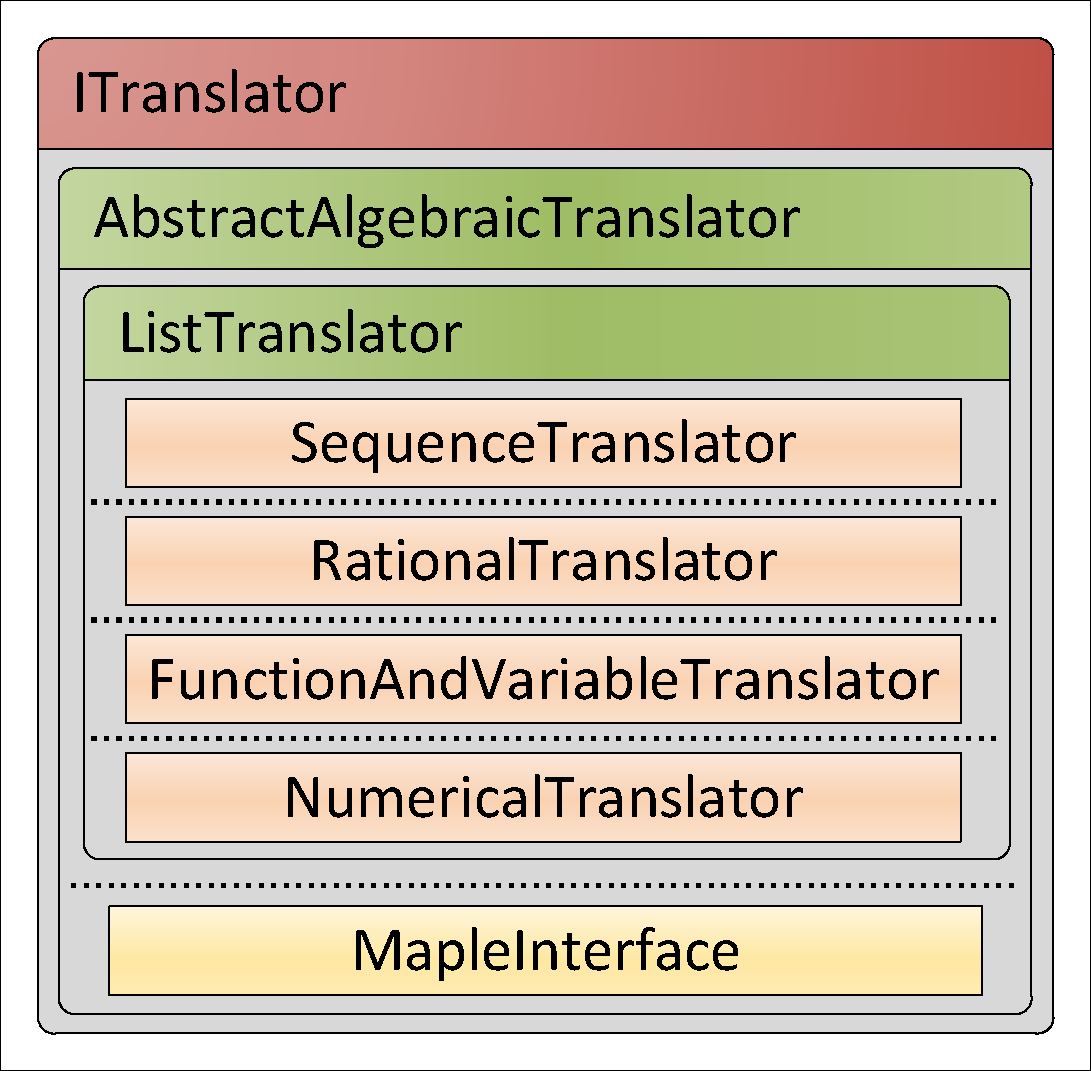
\includegraphics[clip, trim=0.1cm 0.1cm 0.1cm 0.1cm, scale=0.39]{BackwardTranslator.pdf}
	\caption{A scheme of the backward translator and its specialized subtranslators.}
	\label{fig:BackwardDel}
	\vspace{-13pt}
\end{wrapfigure}

The general translation process runs through different states. Each translation process starts with the string representation of a \texttt{1D} \Maple{} input. This string will be converted to the internal nested list representation of our custom \inertF{} (see the previous subsection~\ref{subsec:maple-probs}). Since the \inertF{} is similar to an expression tree, it can be translated as the \gls{mlp-pt} in the forward translation. Hence, we use the same approach of multiple subtranslators for the backward translation process.

Figure~\ref{fig:BackwardDel} shows the subtranslators of the backward translation process. The structure is the same as for the forward translation, seen in figure~\ref{fig:ForwardDel}. The \verb|MapleInterface| represents the entry point of a translation process. Before the translation starts, the \Maple{} kernel needs to be initialized and prepared for the translation process by loading all custom procedures. Once everything is loaded, an expression is delegated to specialized subtranslators depending on the internal data type, defined by custom procedures and \Maple's \inertF.

The following figure~\ref{fig:backward-trans} illustrates the backward translation process for the Jacobi polynomial example $\JacobiP{\alpha}{\beta}{n}@{\cos@{a\Theta}}$ from table~\ref{tab:JacobiP-usecase}. The input expression is converted to the nested list representation of the \texttt{MyInertForm} (the customized \inertF{} of \Maple). Afterwards, each node of the tree is translated separately by specialized subtranslators (visualized by blue arrows). The translation of functions (bold blue arrows) is again realized by translation patterns, which define the correct position for each argument. The last step is used to put all translated arguments to the right position (visualized by red arrows).

\begin{figure}[!htp]
	\centering
	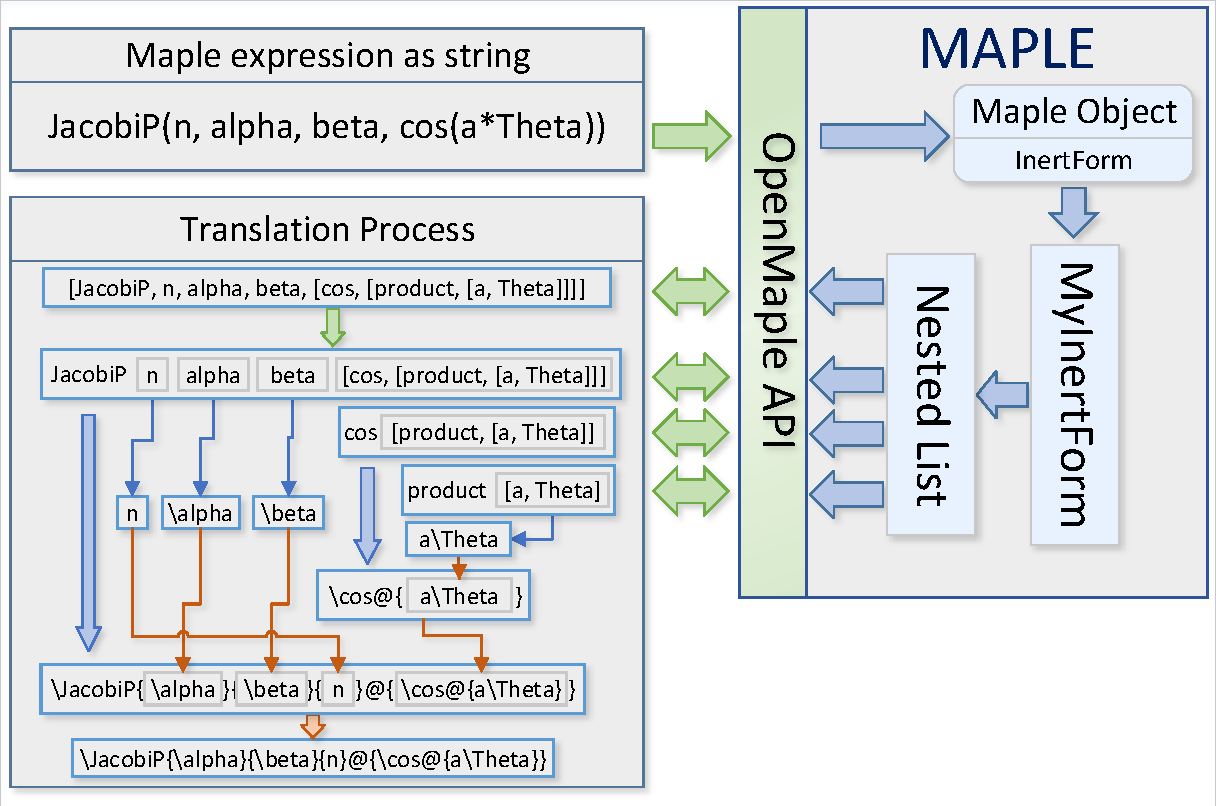
\includegraphics[clip, trim=0.1cm 0.1cm 0.1cm 0.1cm, scale=0.7]{MapleTranslation.pdf}
	\caption{A scheme of the backward translation process from \Maple{} for the Jacobi polynomial $\JacobiP{\alpha}{\beta}{n}@{\cos@{a\Theta}}$. The input string is converted by the \Maple{} kernel into the nested list representation. This list is translated by subtranslators (blue and red arrows). A function translation (bold blue arrows) is again realized by translation patterns to define the position of the arguments (red arrows).}
	\label{fig:backward-trans}
\end{figure}

\cleardoublepage